%!TEX root=../../autopilot.tex
\section{Existing Systems for Behavioral Experiments}
\label{sec:existing}

At minimum, a complete system to automate behavioral experiments has 6 requirements:

\begin{enumerate}

\item \hyperref[sec:hardware]{Hardware}\marginnote{
\includegraphics[]{figures/side_2_hw.pdf}} to interact with the experimental subject, including \textbf{sensors} (eg. photodiodes, cameras, rotary encoders) to receive input and \textbf{actuators} (eg. lights, motors, solenoids) to provide feedback.
\item Some\marginnote{
\includegraphics[]{figures/side_3_stim.pdf}} capability to synthesize and present sensory \hyperref[sec:stim]{stimuli}. Ideally both discrete stimuli, like individual tone pips or grating patches, and continuous stimuli, like those used in virtual reality experiments, should be possible.
\item A \marginnote{
\includegraphics[]{figures/side_4_task.pdf}} framework to coordinate hardware and stimuli as a \hyperref[sec:tasks]{task}. Task definition should be flexible such that it facilitates rather than constrains experimental design.
\item A \hyperref[sec:data]{data management}\marginnote{
\includegraphics[]{figures/side_5_data.pdf}} system that allows fine control of data collection and format. Data should be human readable and include complete metadata that allows independent analysis and reproduction. Ideally the program would also allow some means of realtime data processing of sensor values for use in a task.
\item Some\marginnote{
\includegraphics[]{figures/side_6_viz.pdf}} means of \hyperref[sec:plotting]{visualizing data} as it is collected in order to  observe task status. It should be possible to customize visualization to the needs and structure of the task.
\item Finally,\marginnote{
\includegraphics[]{figures/side_7_ui.pdf}} a \hyperref[sec:ui]{user interface} to control task operation. The UI should make it possible for someone who does not program to operate the system.
\end{enumerate}

We\marginnote[-0.6cm]{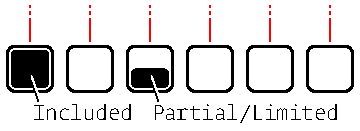
\includegraphics[]{figures/side_8_checks.pdf}} will briefly describe two other systems that meet this definition of completeness: pyControl and Bpod.

%\vspace{16pt}
%\sffamily{\textbf{\Large{pyControl}}}\normalfont
\subsection{pyControl}

\href{https://pycontrol.readthedocs.io/en/latest/}{pyControl}\citep{akamOpensourcePythonbasedHardware2022}\marginnote[0cm]{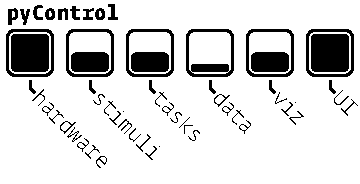
\includegraphics[]{figures/side_9_pyc.pdf}} is a behavioral framework built in Python by the Champalimaud Foundation. It uses the \href{https://micropython.org/}{micropython microcontroller} ("pyboard") as its primary hardware device along with several extension boards \href{http://www.open-ephys.org/store/pycontrol}{sold by openephys}. The pyboard has four I/O ports, or eight with a multiplexing expander board. Schematics are available for many other hardware components like solenoid valve drivers and rotary encoders. Multiple pyboards can be connected to a computer via USB and run independent tasks simultaneously with a GUI.

There is limited support for some parametrically defined sound stimuli, presented from a separate amplifier connected using the I2C protocol. Visual stimuli are unsupported.

Like most behavioral software, pyControl uses a finite-state machine formalism to define its tasks. A task is a set of discrete states, each of which has a set of events that transition the task from one state to another. pyControl also allows timed transitions between states, and one function that is called on every event for a rough sort of parallelism. pyControl also allows the use of external variables to control state logic, making these state machines more flexible than strict finite state machines.

\begin{marginfigure}[-3.5cm]
\begin{minted}[frame=lines,fontsize=\small]{python}
D 0 2
D 8976 3
D 8976 1
P 8976 Print Statement
D 10162 3
D 10163 2
\end{minted}
\caption{pyControl data is stored as plain text, each line having a type (like \textbf{D}ata or \textbf{P}rint), timestamp, and state}
\label{fig:pycdata}
\end{marginfigure}

All events and states are stored alongside timestamps as a plain text log file, one file per subject per session (Figure \ref{fig:pycdata}). Anlog data are stored in a custom binary serialization that alternates 4-byte data and timestamp integers.

There is only one plot type available in the GUI, a raster plot of events, and no facility for varying the plot by task type. The GUI is otherwise quite capable, including the ability to batch run subjects, redefine task variables, and configure hardware.\\

%\sffamily{\textbf{\Large{Bpod}}}\normalfont
\subsection{Bpod}

Bpod\marginnote{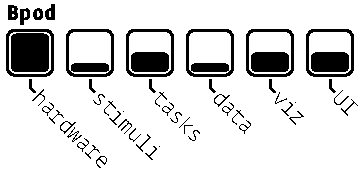
\includegraphics[]{figures/side_10_bpod.pdf}} is primarily a collection of hardware designs and an assembly service run by \href{https://www.sanworks.io/about/about.php}{Sanworks LLC.} Similar to pyControl, each Bpod behavior box is based on a finite-state machine microcontroller with four I/O ports. Additional hardware modules provide extended functionality. Bpod is controlled using its own \href{https://github.com/sanworks/Bpod_Gen2}{MATLAB package}, though there are at least two other third-party software packages, \href{https://brodylabwiki.princeton.edu/bcontrol/index.php/Main_Page}{BControl} and \href{https://pybpod.github.io/}{pyBpod}, that can control Bpod hardware. A task is implemented as a MATLAB script that constructs a new state machine for each trial, uploads it to the Bpod, and waits for the trial to finish. As a result, only one Bpod can be used per host computer, or at least per MATLAB session. Data are stored as trial-split events in a MATLAB structure.

There are a few basic plots for two-alternative forced choice tasks, but there doesn't seem to be a prescribed way to add additional plots. Bpod has a reasonably complete GUI for managing the hardware and running tasks, but it is relatively technical (Figure \ref{fig:bpodgui}).

\begin{marginfigure}
\noindent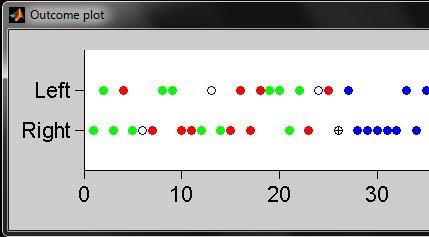
\includegraphics[]{figures/side_11_bplot.jpg}
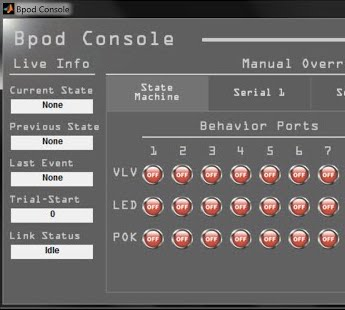
\includegraphics[]{figures/Bconsole.jpg}
\caption{A Bpod event plot (above) showing the results of individual behavioral trials, and the Bpod GUI (below).} 
\label{fig:bpodgui}
\end{marginfigure}


\vspace{16pt}

For brevity we have omitted many other excellent tools that perform some subset of the operations of a complete behavioral system, or otherwise have a substantial difference in scope.\sidenote[][1cm]{\textbf{Other tools:}\\
- Bonsai\citep{lopesBonsaiEventbasedFramework2015b} - \href{https://bonsai-rx.org/}{site}, \href{https://github.com/bonsai-rx/bonsai}{git}\\
- Expyriment\citep{krauseExpyrimentPythonLibrary2014} - \href{https://www.expyriment.org/}{site}, \href{https://github.com/expyriment/expyriment.git}{git}\\
- PsychoPy\citep{peircePsychoPy2ExperimentsBehavior2019} - \href{https://www.psychopy.org/}{site}, \href{https://github.com/psychopy/psychopy}{git}\\
- OpenSesame\citep{mathotOpenSesameOpensourceGraphical2012} - \href{https://osdoc.cogsci.nl/}{site}, \href{https://github.com/smathot/OpenSesame}{git}\\
- SMiLE - \href{https://smile-docs.readthedocs.io/en/latest/}{docs}\\
- ArControl\citep{chenArControlArduinoBasedComprehensive2017} - \href{https://github.com/chenxinfeng4/ArControl}{git}\\
- and see \href{http://openbehavior.com/}{OpenBehavior}
}